\documentclass{article}
\usepackage[utf8]{inputenc}
\usepackage{graphicx}
\usepackage{svg}
% change reference style to [1], remove stupid sorting, language changed so date in ddmmyyyy
\usepackage[backend=biber, style=alphabetic, sorting=none, language=australian]{biblatex}
\addbibresource{References.bib}

\title{Report}
\author{David Saunders (910995)}
\date{April 2020}

\begin{document}
\maketitle

\begin{abstract} 
    Write abstract here. 4 page report!
\end{abstract}

\tableofcontents

\section{Introduction}
%10%
% Contextualise the machine-learning problem and introduce the
% task and the hypothesis. Make sure to include a few references to previous
% work. You should demonstrate an awareness of the research-area.

Image detection is a classic machine learning problem, with hundreds of papers on the topic. 
History of image detection is relatively recent.
Maybe started with the MNIST handwritten digit classification problem.
Is regarded by many as the 'Hello world' of machine learning/CNNs \cite{tensorflow_2020}.
One guy on kaggle used a cnn for the first time to great effect.
Other more advanced problems such as image recognition, gesture
    , emotion detection now possible thanks to deeper networks, and convolution's layers.


Maybe touch on the problem some people have of using too advanced method for the task?
Especially with stuff like pretrained CNN specialised for facial recognition used to detect a black or white dot for example.


\section{Methodology}
%50%
% The model(s) you trained to undertake the task. Any decisions
% on hyperparameters must be stated here, including motivation for your
% choices where applicable. If the basis of your decision is experimentation
% with a number of parameters, then state this.

The training data a classifier will be trained on has the size 51x51x3 where as the images created from the pointcloud have shape 160x240x3, so cannot just be input into a classifier.
Instead a sliding window approach will be used, to split larger image into windows the same size as the training data.   
If a window contains a sphere then the depth of the middle pixel will be recorded.
The windows will overlap strongly so that the set of windows will contain multiple partial spheres \cite{forsyth2002computer}.
The classifier will be trained so that it only recognises a sphere if it is in the centre of an image, therefore the middle pixel will always be the depth.
The camera will then move to the sphere with the lowest depth, which will be the closest sphere.
The X,Y,Z coordinates of the sphere will be found from the middle pixel value for the projected mappings.
If no spheres are detected in any window then the viewpoint will rotate $-\frac{\pi}{6}$ radians in the Y axis until a sphere is detected.

\subsection{Classifier 1: Convolutional Neural Network}

It was decided to use a Convolutional Neural Network (CNN) as a sphere classifier due to their tried and trusted effectiveness at image detection.
Detecting the red sphere is a trivial use of the technology so accuracy is expected to be very high.
Problem will be with the training data not relating to the real life data where the spheres will be obscured and different sizes from the training.
Problem of training/archived data not matching production is a well known issue (with prediction and stuff) TODO: ref.
A benefit of using a CNN is that we do not have to worry about feature extraction, the training data can be input directly into the network.

All of the architecture of the CNN will be explained in this paragraph and all of the hyperparameters explained.
The CNN used in this task is similar to previous Imagenet classification CNN's where there are a series of convolutional and pooling layers
, followed by a fully connected layer \cite{krizhevsky2012imagenet}. 
The architecture used in this CNN is heavily inspired by the LeNet-5 Convolutional neural network, originaly used for handwritten digits recognition.
This architecture was chosen as it is one of the first CNN's to be proposed and it is relatively shallow compared to newer deep learning methods, so training time and memory usage will be less intensive \cite{lecun1998gradient}. 

\begin{figure}[ht]
    \noindent\makebox[\textwidth]
    {%
        \centering
        %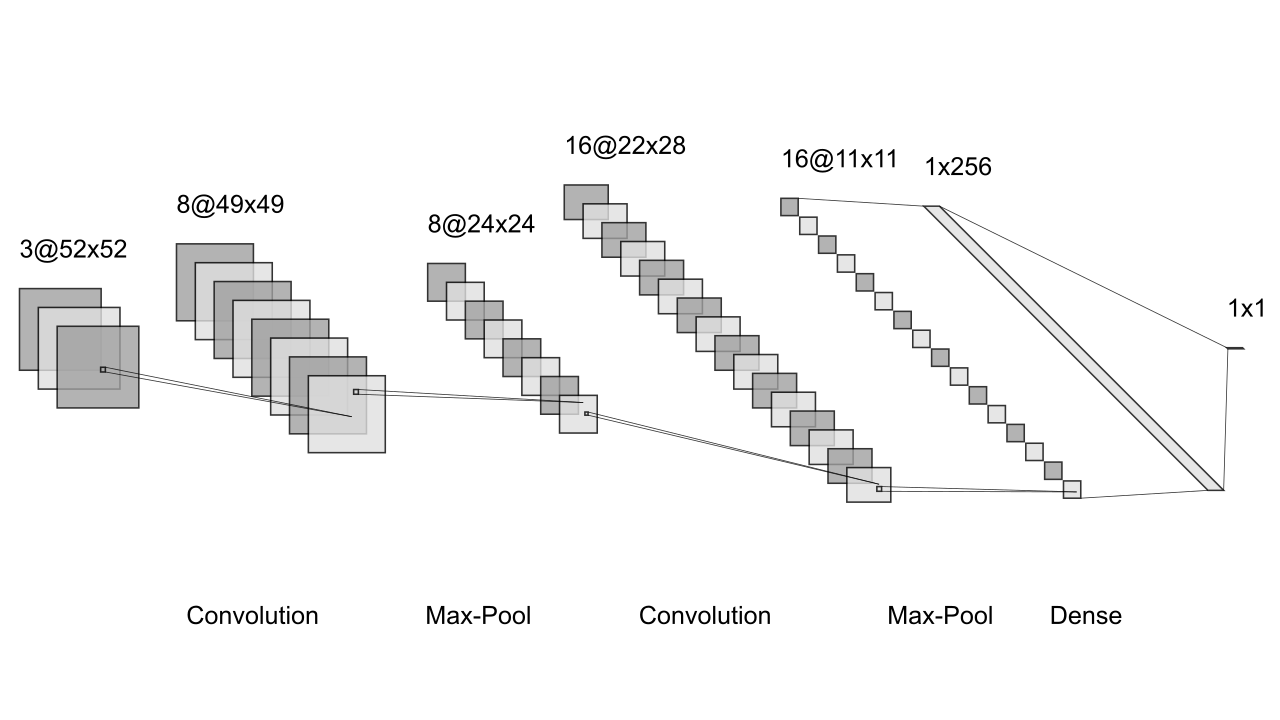
\includegraphics[scale=0.8]{CNN_Zoomed.png}
        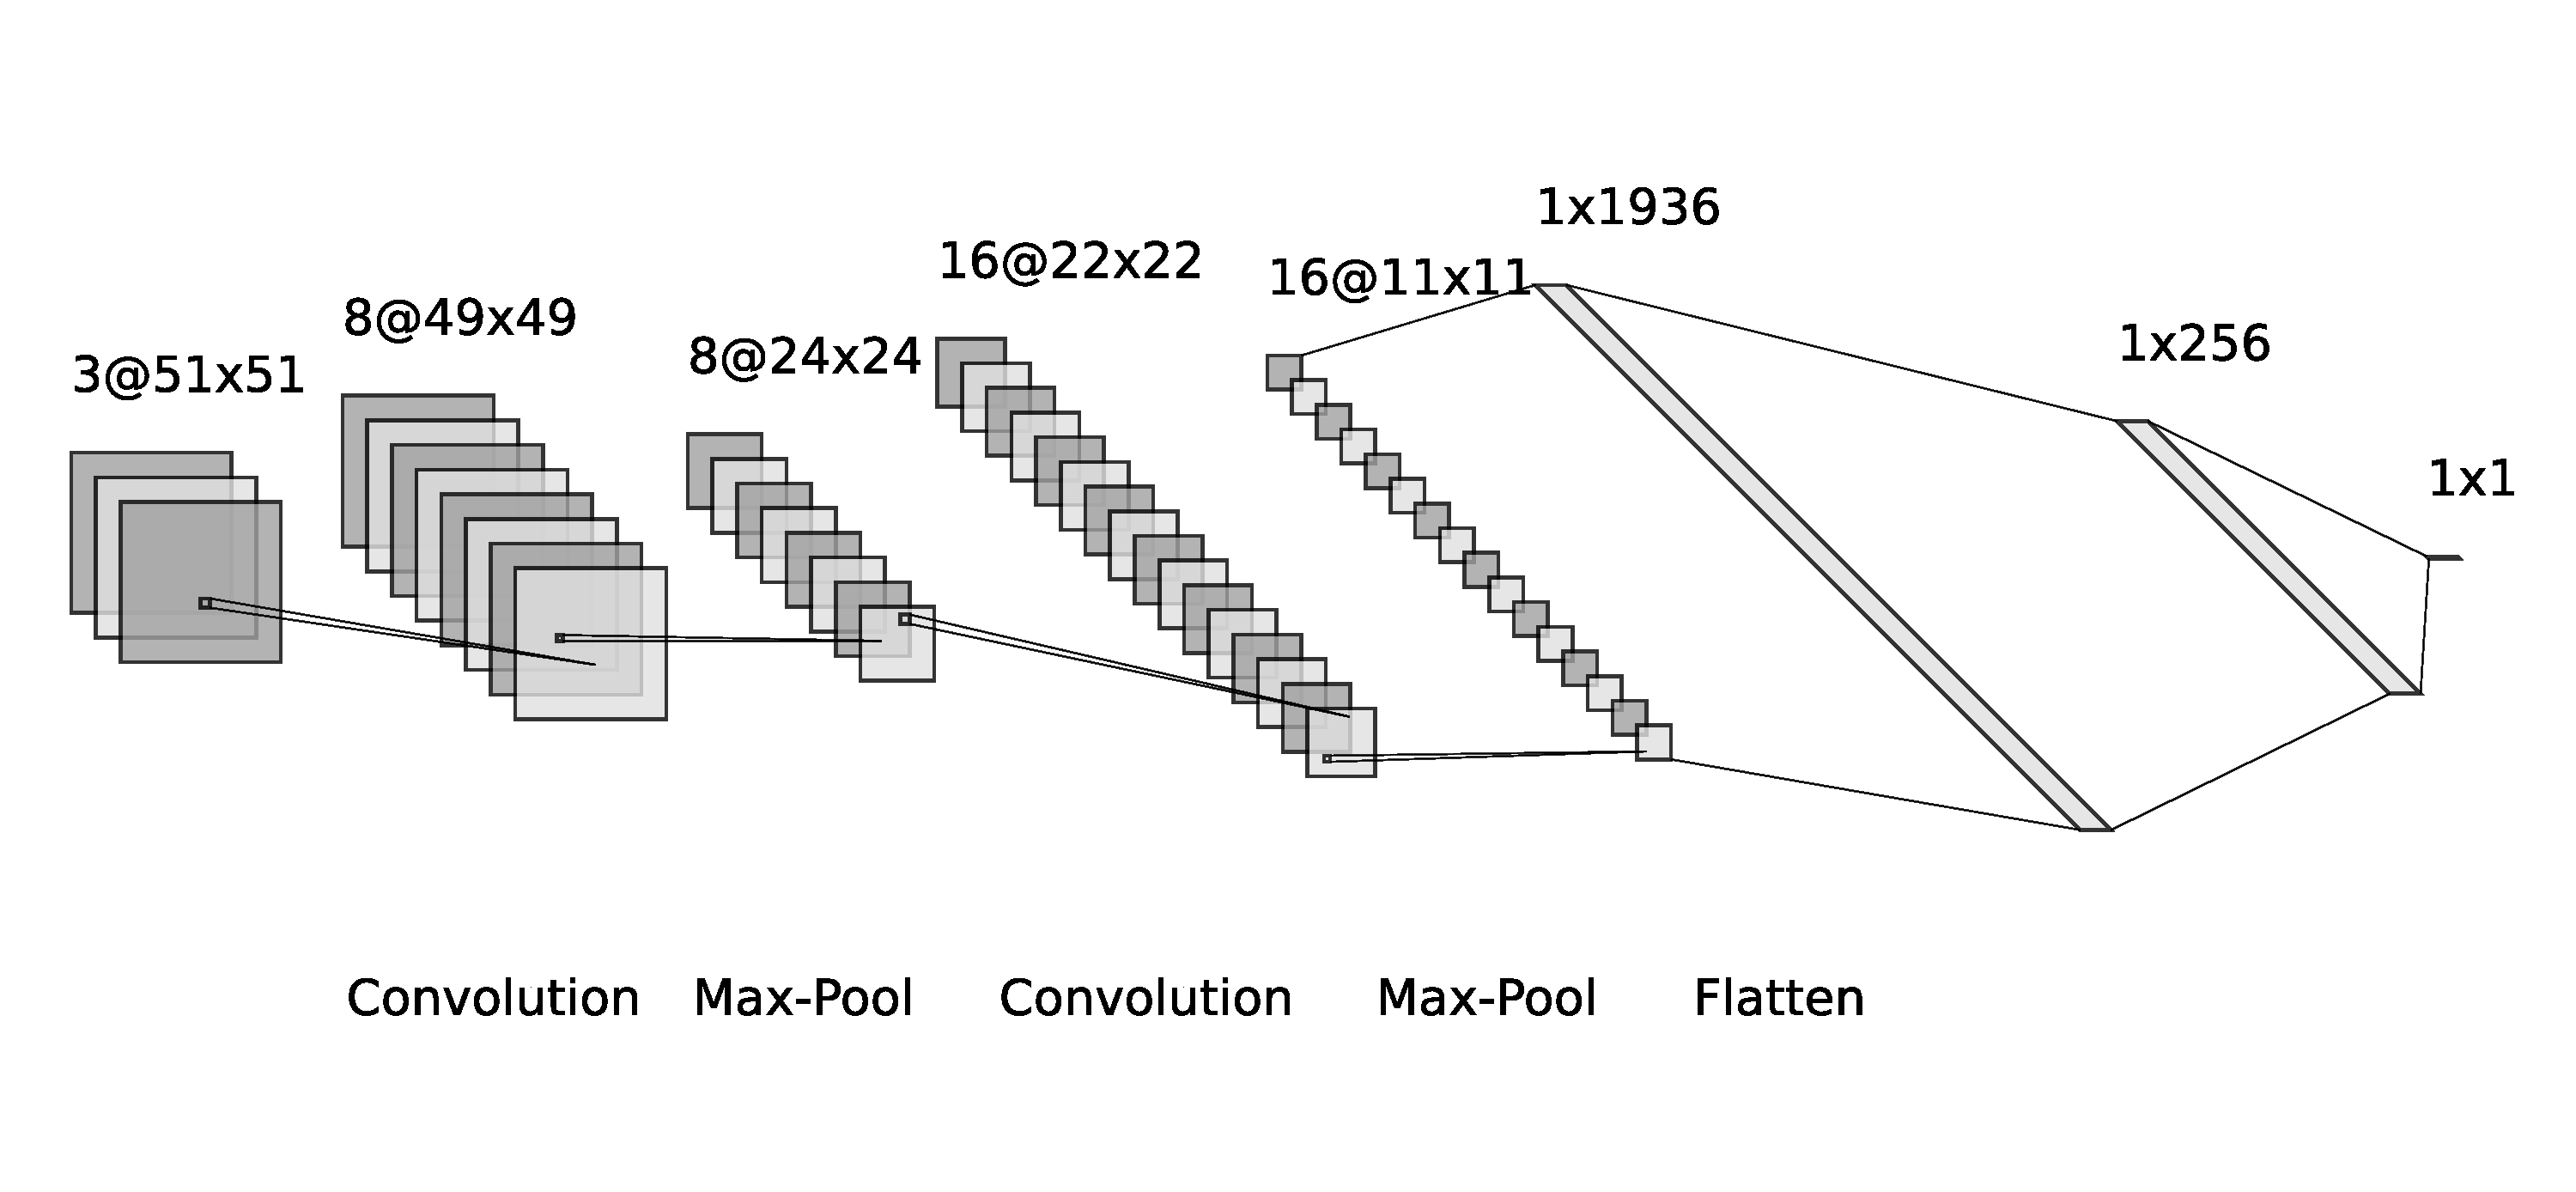
\includegraphics[scale=0.25]{CNN.pdf}
    }
    \caption{A diagram of the network showing the layers \cite{LeNail2019}}
    \label{fig:diagram}
\end{figure}

Figure \ref{fig:diagram} shows the network consists of two convolutional layers
, which are then flattened and fed into  a dense fully connected layer
, which leads to a single output neuron.
Each convolutional layer is followed by a maxpooling layer.
Pooling is used to downsample the image, it is hoped that max pooling will pick up any feature found by the earlier layers.
Why max-pooling is used and not min pooling, or average pooling.
Pooling size is 2, 2 WHY and what exactly does it mean?

All internal nodes of the network use relu as the activation function, other than the output neuron which uses the probability based sigmoid function.
% TODO: explain why relu was chosen? Activation of each internal layers use relu as that is default for whatever reason. Alternative is to use something like sigmoid, but relu is now generally used because xyz. 
The kernel size of the convolutional kernels were chosen arbitrarily as 3x3, and the pooling layers used are 2x2.
Due to the nature of kernel convolutions the input size of each layer will change slightly.
This will be detailed below.

The first convolutional layer takes in a 51x51x3 image, and outputs 8 filters with a reduced size of width and height of 49x49.
The filters are then max pooled to give a new shape of 24x24x8.
The second convolutional layer inputs the downsampled results and outputs a higher number of 16 filters.
The number of filters is increased in an attempt to group together any lower level features that have been identified.
Compared to other image classification tasks this one is trivial so there is no need for more layers to detect low and high level features.
Regardless when a shallower network was tried it didn't work so here we are.  
Pooling after this layer results in an output of shape 11x11x16.
After the convolutional layers we then flatten the output into a vector of length 1936 so that it can be input into a more traditional dense network of nodes.
A layer of 256 neurons is used as the hidden layer, which connects to a single neuron which predicts what class the input image belongs to.
This is given as a probability from 0 (no sphere present) to 1 (sphere present).
Between the hidden and output layers there is a dropout amount specified at 50\%, this means that half of these neurons randomly wont fire.
This method has been shown to reduce overfitting as each hidden neuron cannot rely on another neuron firing \cite{hinton2012improving}. %(weak explanation) 

When training the network the loss function is chosen to be $binary/_crossentropy$ as it is the best choice for binary classification.
Why did I choose rmsprop as an optimizer? 

The data will be trained with 5 epochs, as it is believed this will be sufficient to maximise accuracy, but prevent overfitting.
Obviously an epoch is a full pass through the dataset and we're only given a small dataset to work with so overfitting is the biggest worry.
TODO: Reference of course.
\url{machinelearningmastery.com/early-stopping-to-avoid-overtraining-neural-network-models/}
This article list loads of nice academic sources about how to avoid overfitting.

The model is then saved to disk as a $.hdf5$ file.
This is so the network doesn't have to be retrained all the time and to help reproducibility.
(Get reference to why you should always save a model)
Since networks are non-deterministic they may not always have the same result (ref).

\subsection{Classifier 2: Dummy classifier}
CNN is good and all but is it too complicated for the job?

while messing around it was found that multiple layers were needed to properly classify the spheres.
Could manual feature engineering help? (Feature engineering is a good word just TODO: find reference.)
In the training data the red sphere is always in the centre, with the center pixel having a very high red intensity, with a low intensity for the green and blue channels. 
Idea was that by using human knowledge to extract features using domain knowledge could prove just as effective as state of the art machine learning.
Perhaps there'd even be benefits of a computational speedup when a more simple method was used.


\section{Results}
% 30%
% Describe, compare and contrast the results you obtained on your
% model(s). Any relationships in the data should be outlined and pointed
% out here. Only the most important conclusions should be mentioned in
% the text. By using tables and confusion-matrices to support the section,
% you can avoid describing the results fully.

The methods of completing the PacMan game as discussed above were successful when the CNN architecture was used.
The main for loop of the program ran for a time of 12 minutes, and every sphere was detected and moved to flawlessly.
The time is high however that is not because of the classifier used but rather the function of projecting the point cloud to the 5 different maps that bottlenecked the system.
Neural networks are even known for their speed of classification once they've been trained.

Confusion matrix of CNN:
(Only text or with a nice graph)


As discussed NNs are fast at classification, but how does that compare to an even simpler method of classification.
To complete the game using the dummy classifier took only 9 minutes.
Despite the classifier not being the bottleneck, there was a notable speed increase.
One possible explanation for the speedup is that the dummy, classifier is less robust and adaptable to channge than the CNN.
Sphere would have to be directly in centre of screen, meaning less spheres were identified and so less things to process?
TODO: Look at results to see if this theory holds any weight at all.

TODO: time both classifiers on the same starting test image, and then sliding windows classifier measured to compare time differences.


Confusion matrix of dummy:
(Only text or with a nice graph)


\section{Discussion and Conclusion}
% 10%
% Restate the task and hypothesis/-ses concisely.
% Reiterate the methods used. Describe the outcome of the experiment
% and the conclusion that you can draw from these results in respect of the
% hypothesis/-ses.

Task at hand was a simple binary image classifier that was to be used in conjunction with other methods to play a game moving thorough 3D space.
A CNN was used as they are the de facto, tried and tested method of dealing with this problem.
Despite this a simple dummy classifier was created using manual feature extraction which performed just as well.
This shows how there is not always a need for the most advance options and that given some knowledge of the problem, manual feature engineering can be the most effective.

\printbibliography

\end{document}